\documentclass{article}

% If you're new to LaTeX, here's some short tutorials:
% https://www.overleaf.com/learn/latex/Learn_LaTeX_in_30_minutes
% https://en.wikibooks.org/wiki/LaTeX/Basics

% Formatting
\usepackage[utf8]{inputenc}
\usepackage[margin=1in]{geometry}
\usepackage[titletoc,title]{appendix}
\usepackage{hyperref}
\hypersetup{colorlinks=true}

% Math
% https://www.overleaf.com/learn/latex/Mathematical_expressions
% https://en.wikibooks.org/wiki/LaTeX/Mathematics
\usepackage{amsmath,amsfonts,amssymb,mathtools}

% Images
% https://www.overleaf.com/learn/latex/Inserting_Images
% https://en.wikibooks.org/wiki/LaTeX/Floats,_Figures_and_Captions
\usepackage{graphicx,float}
\usepackage{caption}
\usepackage{subcaption}
\usepackage[section]{placeins}

% Tables
% https://www.overleaf.com/learn/latex/Tables
% https://en.wikibooks.org/wiki/LaTeX/Tables

% Algorithms
% https://www.overleaf.com/learn/latex/algorithms
% https://en.wikibooks.org/wiki/LaTeX/Algorithms
\usepackage[ruled,vlined]{algorithm2e}
\usepackage{algorithmic}

%% Code syntax highlighting
%% https://www.overleaf.com/learn/latex/Code_Highlighting_with_minted
%\usepackage{minted}
%\usemintedstyle{borland}
\usepackage{listings}

% References
% https://www.overleaf.com/learn/latex/Bibliography_management_in_LaTeX
% https://en.wikibooks.org/wiki/LaTeX/Bibliography_Management
\usepackage{biblatex}
\addbibresource{references.bib}

% Title content
\title{Market Price Sensitivity to News}
\author{Jason Sawyer}
\date{March 16, 2020}


\begin{document}

\maketitle

% Abstract
\begin{abstract}
In the age of information, we are flooded with news articles every day that can be accessed virtually anywhere and at anytime given the proliferation of smartphones, laptops, and traditional media.  Investors pay close attention to the news.  When recent developments impact their economic forecasts, they make trading decisions that directly impact stock prices.  Therefore, to some extent stock prices can be thought of as a function of the news.  Is it possible, then, to forgoe fundamental analysis of the economy and instead directly model this relationship to predict market movements?  In this paper, we will consider this question from a mathematical perspective.  We will leverage techniques for natural language processing, dimension reduction, and machine learning classification to attempt to describe this relationship.
 \\
\begin{center}
\href{https://github.com/sawy0056/TextAnalysis}{\color{blue}{https://github.com/sawy0056/TextAnalysis}}
\end{center}
\end{abstract}

% Introduction and Overview
\section{Introduction and Overview}
Theoretically, the price of a stock represents the true value of a company driven by its fundamental financial health.  Market participants constantly update their assumptions and reevaluate their positions.  For example, suppose that a major news outlet reports that holiday sales are significantly lower than in previous years.  Stock traders would likely react by lowering their expected earnings forecasts for major retailers which would in turn drive their stock prices lower.  

As another example, consider the uncertainty surrounding the novel coronavirus.  As news coverage pours out on a daily basis, market participants are unsure how to forecast the full economic impact.  Surely, there will be disruption to international supply chains and likely a domestic slowdown if more extreme quarantine measures become necessary in the U.S.  The anxiety surrounding this has manifested in drastic market corrections and significant volatility. 

These are two examples of how analysts leverage news to recalculate their outlook on fundamental valuations of companies.  In addition to analysts, of course there is a growing portion of trade volume being driven by algorithms.  Many of these algorithms trade on momentum and, at times, serve to amplify market swings.  

All of the above begs the question; it is possible to construct a model that predicts the market’s reaction to the latest news?  In this paper, we will consider this question with the following approach.  First, we will construct a web crawler to gather raw text from news articles over a historical window.  Second, we will analyze this text data by leveraging concepts from natural language processing.  Finally, we will use the singular value decomposition coupled with machine learning techniques in an effort to predict market movements.





%  Theoretical Background
\section{Theoretical Background}
The two primary tools employed in this research are the singular value decomposition (SVD) and the Linear Discriminant Analysis (LDA).

\subsection{Singular Value Decomposition}
The singular value decomposition (SVD) is one of the most powerful results in linear algebra.  Given a matrix of data, the SVD will provide information about both the direction and magnitude of its covariance.  

\begin{equation}
M = USV^*
\end{equation}


Geometrically, the SVD is a rotation (U), a stretch (S), and another rotation (V).  Both U and V are unitary real or complex matricies that need not be square while S is a diagonal matrix containing the singular values.  

The goal of the SVD is to take the matrix M into a new coordinate system in which the variance of the system is orthogonalized.  In other words, all correlations have been accounted for and only the truly distinct directions of variance remain.  Suppose an array of 10 points over time were perfectly correlated.  The SVD would determine that all variation to this system can be explained with a single mode representing parallel shifts.  The dimension of this system would thus be reduced from 10 to 1.

\begin{figure}
    \centering
    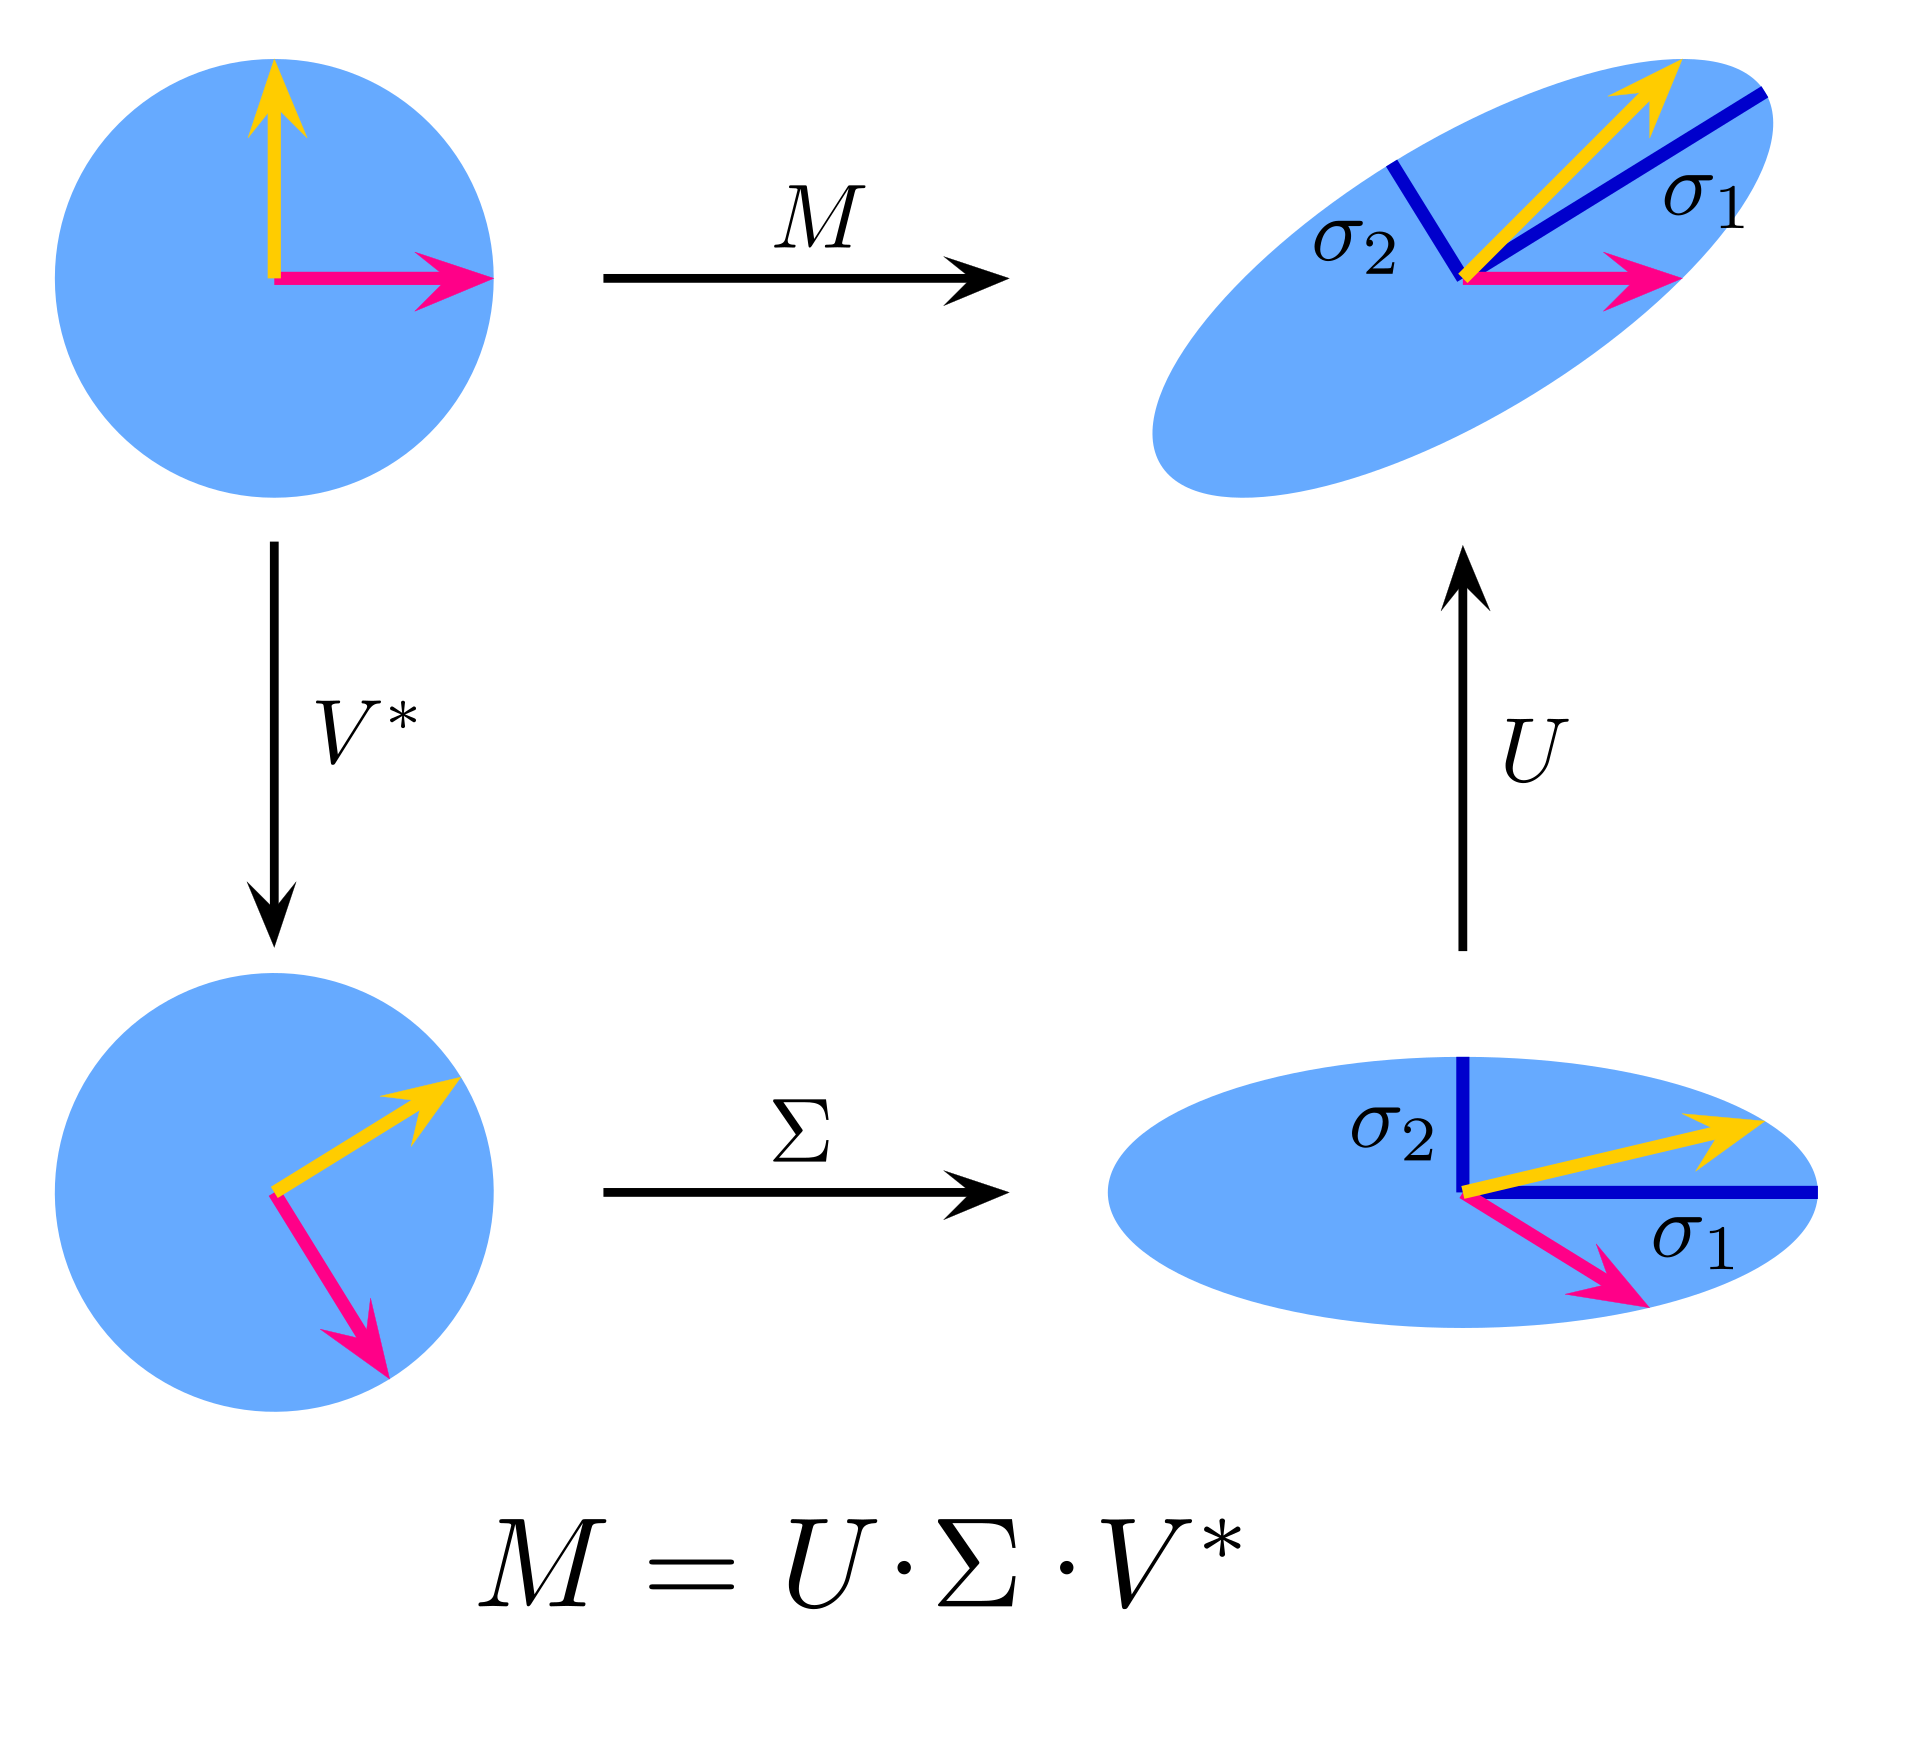
\includegraphics[width=0.5\linewidth]{Figures/SVD.png}
    \caption{A geometrical interpretation of the SVD.  Credit to Georg-Johann for producing this image and making it available on wikipedia.  (https://commons.wikimedia.org/wiki/User:Georg-Johann)}
    \label{fig:CumulativeVariance}
\end{figure}


\subsection{Linear Discriminant Analysis}
Given a data set representing two or more classes, linear discriminant analysis seeks a basis that accomplishes two things.  First, the variance within classes are minimized.  In other words, in this new basis the data for each class cluster near each other to the maximum extent possible.  Second, the variance between classes are maximized.  Said another way, while the classes are clustered tightly together with the first condition, the distinct clusters are maximally seperated.  

Mathematically, LDA is defined as

\begin{equation}
w = arg \max_{w} \frac{w^{T}S\textsubscript{B}w}{w^{T}S\textsubscript{W}w}
\label{eqn:LDA}
\end{equation}

Having $S\textsubscript{W}$ in equation \ref{eqn:LDA} defined as

\begin{equation}
S\textsubscript{W} = \sum\limits_{i=1}^{C} S\textsubscript{i} 
\end{equation}

With $S\textsubscript{i}$ as
\begin{equation}
S\textsubscript{i} = \sum\limits_{z \in w\textsubscript{i}} (x-\mu\textsubscript{i})(x-\mu\textsubscript{i})^T
\end{equation}

\begin{equation}
\mu\textsubscript{i} = \frac{1}{N\textsubscript{i}}\sum\limits_{z \in w\textsubscript{i}} x
\end{equation}


$S\textsubscript{B}$ in equation \ref{eqn:LDA} is defined as follows

\begin{equation}
S\textsubscript{B} = \sum\limits_{i=1}^{C} N\textsubscript{i}(\mu\textsubscript{i}-\mu)(\mu\textsubscript{i}-\mu)^T
\end{equation}

Having $\mu$ and $\mu\textsubscript{i}$ defined as

\begin{equation}
\mu = \frac{1}{N}\sum\limits_{\forall x}{ } x = \frac{1}{N}\sum\limits_{\forall x} N\textsubscript{i}\mu\textsubscript{i}
\end{equation}

\begin{equation}
\mu\textsubscript{i} = \frac{1}{N\textsubscript{i}}\sum\limits_{x \in \omega \textsubscript{i}} x
\end{equation}


Given the projection of our data onto this new basis, it should be the case that our data is maximally separated.  With this maximal separation, class boundaries can be drawn such that data within each separate interval represent a distinct class.  Certainly, when working with noisy `real world' data, the effectiveness of this approach will depend completely on the presence of distinct classes.  If there is significant overlap in data, no matter which basis we project onto it will be difficult to achieve satisfactory accuracy in classification predictions.


% Algorithm Implementation and Development
\section{Algorithm Implementation and Development}

Code has been developed in python for this research and is broken into two primary sections.  First, a web crawler has been constructed to gather text data.  Second, given a populated database of text data there is a distinct code base for analysis, plotting, and classification purposes.


\subsection{Web Crawler}
Text data is central to this analysis.  In python, a web crawler has been developed to retrieve every news article from Yahoo Finance for a given day.  This web crawler can be run over many days to accumulate a time series of text data.  While New York Times, Bloomberg, and other publications might also be desired, Yahoo Finance was selected because of simplicity.  
\subsubsection{Workflow}
First, we gather an inventory of article URLs for a news day.  To accomlish this, the Yahoo Finance site map is traversed using the urllib3 and BeautifulSoup libraries.  The raw html from the site map is parsed and only valid news articles are extracted.  

Second, given the inventory of article URLs for a day, we extract the article text for each.  Within a loop, the raw html for each article URL is parsed to locate the article text.  This exercise is surprisingly non-trivial given the overwhelming number of advertisements, script, and style elements embedded throughout the raw html of a typical article URL.  

Third, by leveraging the Natural Language Toolkit (NLTK), the raw text is normalized.  Normalization consists of removing punctuation, capitalization, and stop words such as ‘the’, ‘and’, and ‘of’.  A current list of English stop words are available for download via the NLTK.  After this step, we should be left with a clean list of meaningful words in a given article.  For example, the words ‘rally’, ‘buy’, and ‘optimism’ might remain giving a clear positive sentiment for this particular article.

Fourth, we condense our normalized data into a unique word list paired with the frequency of occurrence.  In other words, which words occurred in this article (the dictionary) and how many times did each word occur (the frequency)?  This vectorized form of text data is ultimately the final form for this analysis.  In future research, the tokenization of word groups and word coincidence would likely prove fruitful.

Finally, to more scientifically assign sentiment to words, the \href{https://hlt-nlp.fbk.eu/technologies/sentiwords}{\color{blue}{SentiWords}} resource has been leveraged.  This resource contains more than 150,000 words and word combinations with an assigned sentiment polarity between -1 and 1.  Positive values are associated with positive sentiment and negative values with negative sentiment.  Greater absolute values represent stronger sentiments.

This workflow is iterated for every article in a news day.  The results of this iteration are combined into one vector per day.  Said another way, we will leverage this crawler to construct a matrix that is (number of distinct words) x (number of dates) in size where each element in the matrix is the frequency of occurrence.

\subsubsection{Crawling Efficiency}
There are an astounding number of articles published in a single news day.  Throughout 2019 and into 2020, it is common for more than 1500 articles, and in some cases well over 2000 articles to be published in a single news day.  Realistically, if leveraging a single threaded approach, the processing time required to gather this data over a meaningful length of history is several months or more.  It is for this reason that a multithreaded approach has been considered.  

It is essential, however, to attempt this multithreaded approach in the most respectful manner possible.  While Yahoo Finance typically fields 150 million site requests per month, hammering their site with several hundred thousand additional requests might put undue burden on their servers.  It is for this reason that a time window from 2013 to 2015 was selected.  Far fewer articles were published per day during this time period which allows us to obtain a fairly long time series to work with for this research while minimizing the additional traffic to Yahoo.
\subsubsection{SQL Database and Threading}
\label{SQL}
A local instance of Microsoft SQL Express was installed for the purpose of storing and accessing the word dictionary, frequencies, and sentiment score data.  Primarily, the need for SQL arose from the threading approach.  As each web crawling thread synchronously retrieves data, a tool that can properly handle the potential need for simultaneous access is required.  For example, a raw text file with the windows operating system does not have the concept of queueing.  SQL Server is designed precisely for this purpose.  

Although threading primarily drove the use of SQL, it additionally performs well as a data transformation and retrieval mechanism for the subsequent analysis.

\subsection{Market Data Sourcing}
Historical market data was downloaded from Yahoo Finance by leveraging their web interface manually.  The csv files were subsequently loaded into the SQL database noted in section \ref{SQL}.


\subsection{Classification}
The classification algorithm implements the core theoretical foundation of this paper.  Specifically, we are classifying a news date as either `buy' or `sell'.  In the `buy' case, we expect that today's daily return will be positive.  In the `sell' case, we expect that today's daily return will be negative. 
 
In order to accomplish this, first the singular value decomposition (SVD) is computed on the text frequency data.  Secondly, given a specified number of principal components to use in the `num features' variable, the modes for each class are extracted.  Supposing a clear difference exists, these modes should capture the unique component signature between days when the market increases versus when it decreases.

The next step is to implement linear discriminant analysis.  This consists of finding the interclass variance, which we’d like to minimize, and the between-class variance which we’d like to maximize.  Given this we can calculate the eigendecomposition by using the ${\it eig()}$ function in SciPy's linear algebra library.  The result of this step should provide us with the linear operation that optimally projects our data into a space where classes are most separated.

The final step is to then draw the boundaries between the separated classes.  These boundaries represent the result of our supervised learning.  With these boundaries we can find our training accuracy to determine how well this approach is performing on the training data.


\begin{figure}
    \centering
    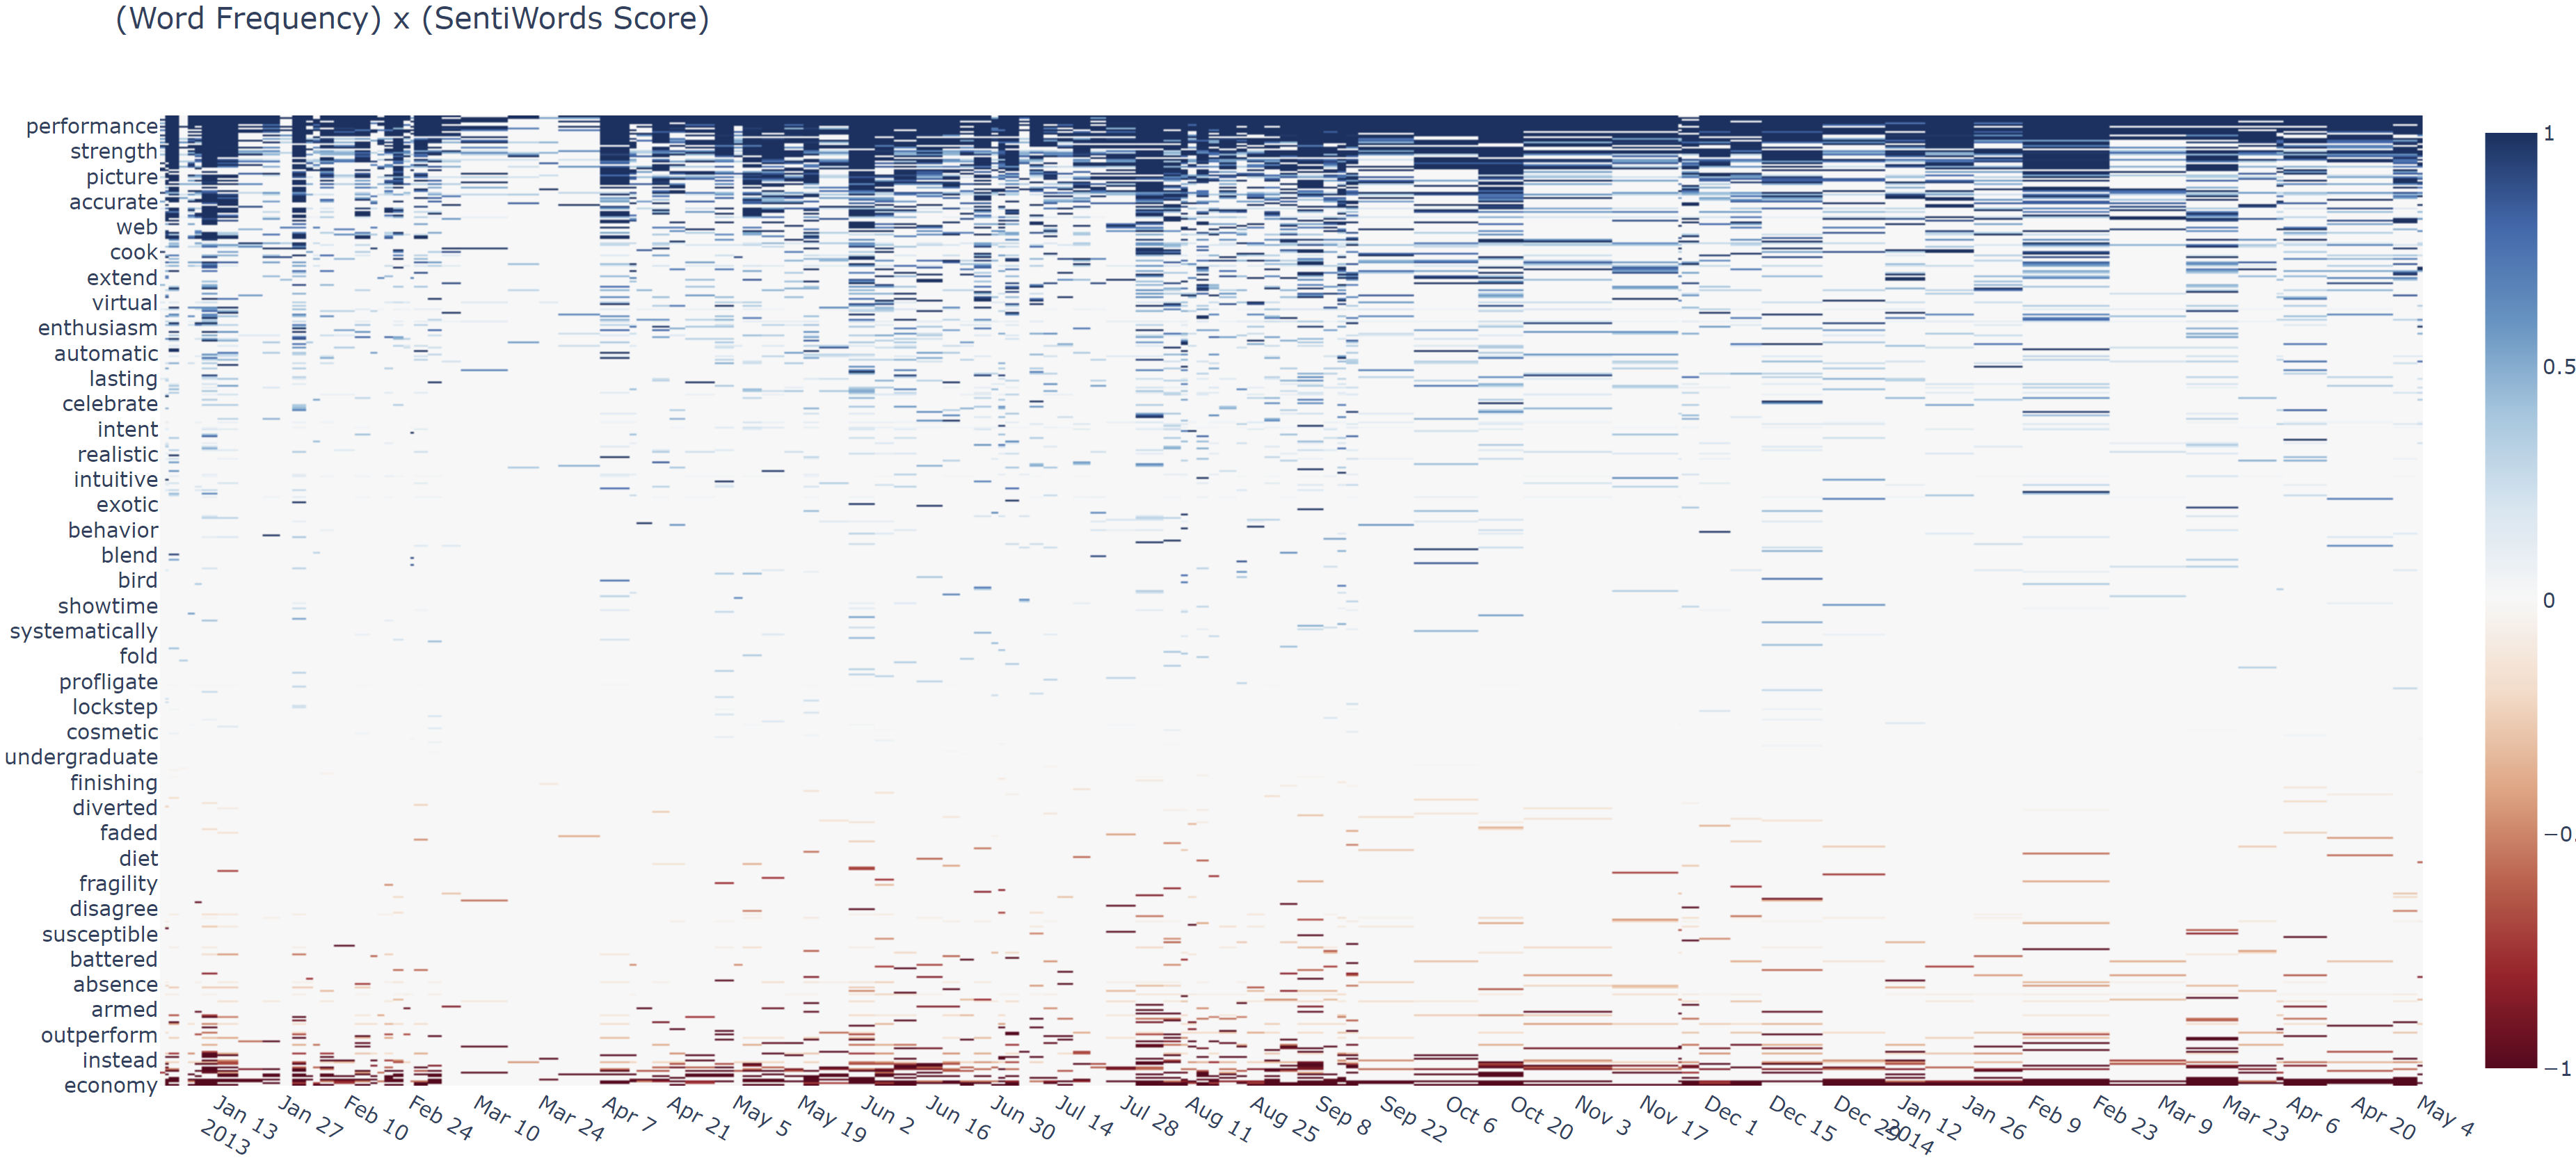
\includegraphics[width=1.0\linewidth]{Figures/0FrequencyMap.png}
    \caption{This heat map represents the dictionary of distinct words that occurred over the historical period.  The color of each cell represents the percent of total frequency per day multiplied by its SentiWords score.  Using this approach, the sentiment of a particular word is captured and it is further weighted by the number of occurrences.  Red represents negative sentiment while blue represents positive sentiment.}
    \label{fig:FreqHeat}
\end{figure}

\section{Computational Results}

A random sample of 98 news days spanning from January 1st, 2013 to May 4th, 2014 has been scraped from Yahoo Finance.  A representation of the word frequencies and sentiments can be seen in figure \ref{fig:FreqHeat}.  In total, after text normalization 23,956 distinct words occurred more than once per day during this time period.  Words occurring only 1 time per day were filtered out due to the increased computing power required to manage the larger data set coupled with the relatively low level of information provided by them.

\subsection{Market Data}
Market data for 6 major indexes and stocks were retrieved from Yahoo Finance and converted to buy versus sell signals.  A representation of these classes can be found in figure \ref{fig:BuySell}.

\begin{itemize}
	\item \texttt{FB} is Facebook stock.  Selected because it was referenced often during this time period.
	\item \texttt{MSFT} is Microsoft stock.  Selected because it was referenced often during this time period.
	\item \texttt{EURUSD} is the Euro to US Dollar exchange rate.
	\item \texttt{VIX} is an index capturing equity market volatility.
	\item \texttt{S\&P} is the S\&P500 stock market index.
	\item \texttt{DJI} is the Dow Jones Industrial Average.
\end{itemize}


\subsection{Test and Training Data}
The text and market data were split into training sets (80\%) and test sets (20\%) for purposes of avoiding data snooping while building the machine learning classifier.

\subsection{Singular Value Decomposition}
Performing the SVD on the training text data, in figure \ref{fig:SVDVar} we find that the text data is well represented with as few as 20 modes.  This is a significant reduction in overall dimension of our text data.. 

\subsection{Classification}
In terms of classification results, the LDA performed surprisingly well on the training data given that a sufficient number of principal components were used in the SVD.  In figure \ref{fig:LDAVarAll}, we find that given a single principal component, the classification is no better than random guessing hovering around 50\% for all indexes and stocks.  

However, on the other end of the spectrum, if leveraging at least 40 modes in the SVD, the Dow Jones Industrial Average, S\&P500, VIX Volatility indicator, and Microsoft stock are all predicted with greater than 90\% accuracy.  In fact, above 60 modes all are predicted with greater than 90\% accuracy while the S\&P500 is predicted with a surprising 100\% accuracy.  A more detailed view of the classification performance for the Dow Jones Industrial Average can be seen in figure \ref{fig:DJIprog}.

\subsection{Test Performance}
On the test data, out of sample performance was less impressive.  As seen in figure \ref{fig:TestPerf}, no index exceeded 80\% accuracy while the majority hovered slightly above guessing at 50\% to 60\%.  One possible reason for this is that the test data set is just too small.  With only 20 days of frequency data represented, we have a very small sample from which to draw conlclusions.  In subsequent work, it will be interesting to allow the web crawler to gather a much longer time series of text data.  Perhaps this will allow for better out of sample performance.

Another possibile explanation for the poor test performance is that this analysis requires a much larger training data set in order to capture the full variation that exists in the universe of news.  In other words, an incredibly wide variety of topics may be covered week to week and month to month.  If we have not included a sufficient sample of this variety in our training, we may not be surprised to see that the algorithm struggles to achieve peak accuracy.  Interpolation given a large training set can often be very successful while extraplation can be much less predictable. 



\begin{figure}
    \centering
    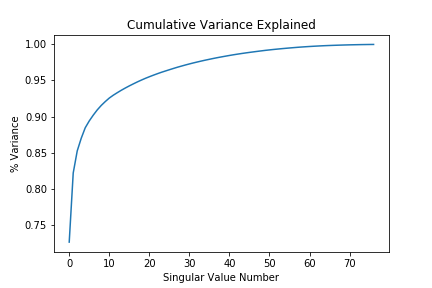
\includegraphics[width=0.5\linewidth]{Figures/SVD_Variance_ExplainedDJI.png}
    \caption{95\% of the variance in the text data, which is comprised of 23,956 distinct words over 98 days, can be represented by 20 principal components.}
    \label{fig:SVDVar}
\end{figure}
\begin{figure}
    \centering
    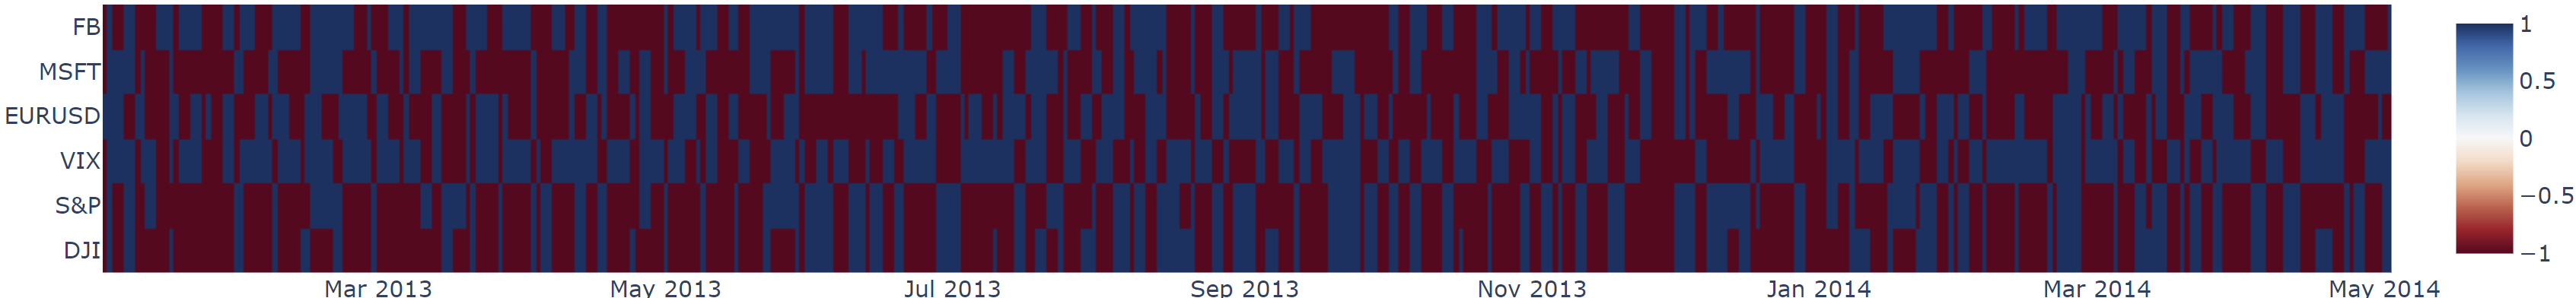
\includegraphics[width=1.0\linewidth]{Figures/BuySellPlot2.png}
    \caption{This heat map represents the buy (blue) and sell (red) signal for 6 market indexes stocks over the historical window.  Buy signals represent positive forward looking daily returns.  Sell signals represent negative forward looking daily returns.  Note that weekends and holidays have been carried forward.}
    \label{fig:BuySell}
\end{figure}
\begin{figure}
    \centering
    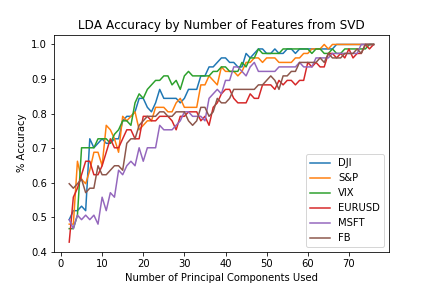
\includegraphics[width=0.5\linewidth]{Figures/LDA_Accuracy_ALL_By_Num_Feature.png}
    \caption{A representation of LDA {\bf training} accuracy performance for each index and stock spanning a range of principal components used in the SVD.}
    \label{fig:LDAVarAll}
\end{figure}
\begin{figure}
    \centering
    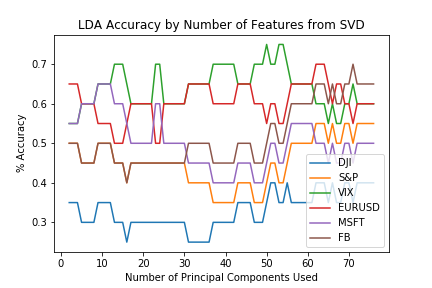
\includegraphics[width=0.5\linewidth]{Figures/Test_Accuracy_ALL_By_Num_Feature.png}
    \caption{A representation of LDA {\bf test} data accuracy for each index and stock spanning a range of principal components used in the SVD.}
    \label{fig:TestPerf}
\end{figure}


\begin{figure}
\centering
%\textbf{Results - Test Case 1 - Ideal}\par\medskip
\begin{subfigure}{.5\textwidth}
    \centering
    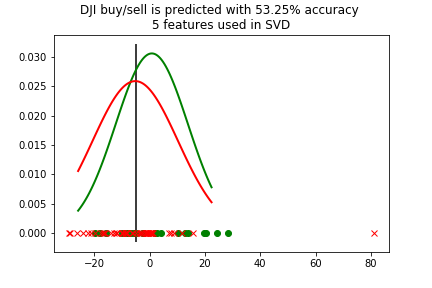
\includegraphics[width=1.0\linewidth]{Figures/LDA_Accuracy_DJI_5.png}
    \caption{ }
    \label{fig:cropVar}
\end{subfigure}%
\begin{subfigure}{.5\textwidth}
    \centering
    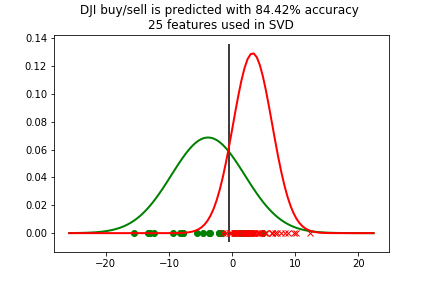
\includegraphics[width=1.0\linewidth]{Figures/LDA_Accuracy_DJI_25.png}
    \caption{ }
    \label{fig:uncropVar}
\end{subfigure}
\begin{subfigure}{.5\textwidth}
    \centering
    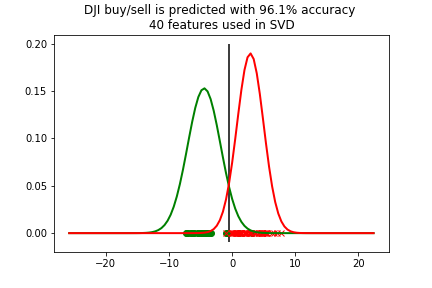
\includegraphics[width=1.0\linewidth]{Figures/LDA_Accuracy_DJI_40.png}
    \caption{ }
    \label{fig:cropVar}
\end{subfigure}%
\begin{subfigure}{.5\textwidth}
    \centering
    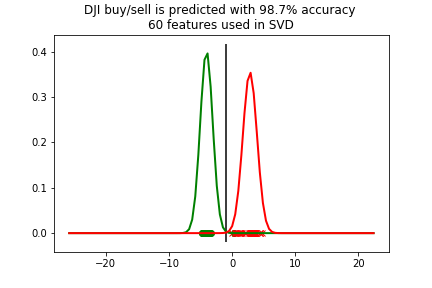
\includegraphics[width=1.0\linewidth]{Figures/LDA_Accuracy_DJI_60.png}
    \caption{ }
    \label{fig:uncropVar}
\end{subfigure}
%\begin{subfigure}{.5\textwidth}
%    \centering
%    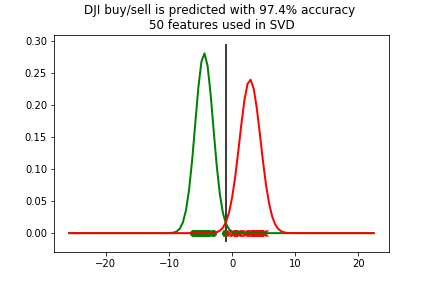
\includegraphics[width=1.0\linewidth]{Figures/LDA_Accuracy_DJI_50.png}
%    \caption{ }
%    \label{fig:cropVar}
%\end{subfigure}%
%\begin{subfigure}{.5\textwidth}
%    \centering
%    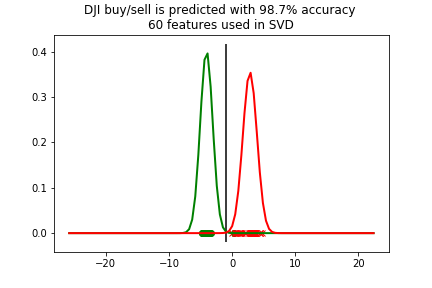
\includegraphics[width=1.0\linewidth]{Figures/LDA_Accuracy_DJI_60.png}
%    \caption{ }
%    \label{fig:D}
%\end{subfigure}


\caption{A visual representation of the LDA applied to the Dow Jones Industrial Average classification.  Green represents the `buy' class while red represents the `sell' class.  The LDA struggles with fewer SVD features but performs exceptionally well in separating the classes when greater than 25 features are used.}
\label{fig:DJIprog}
\end{figure}


% Summary and Conclusions

\section{Summary and Conclusions}

There appears to be a promising relationship present in this research.  Intuitively, the stock market can be thought of as a function of the news and the results presented in this paper suggest that this relationship can likely be quantified.  The linear discriminant analysis (LDA) performed exceptionally well on the training data given a sufficient-rank approximation of the text data.  Less than rank 25 does not produce acceptable results while greater than 50 seems to produce an impressive accuracy.

Test performance paled in comparison to the training performance.  Likely this was driven, at least in part, by a relatively small number of days available for validation.  

Web crawling is a non-trivial exercise.  Developing an algorithm to properly scrape article text from an array of URLs proved more time consuming than anticipated.  In addition, the run time of the web crawler proved significantly longer than expected.  As a result, while a fairly large volume of articles were retrieved in order to form the basis of this analysis, more text data is likely required for a truly robust evaluation.  Since the crawler is fully automated, it can be run perpetually in the background accumulating data to be prepared for future analysis.


 


% References
\printbibliography

\newpage
% Appendices
\begin{appendices}


% MATLAB Functions

\section{Python Functions}
\label{MatlabAppendix}
The following Python libraries and  functions were used for the implementation of the solution to this problem
\begin{itemize}

	\item \texttt{pandas.DataFrame} provided the standard data structure for this analysis.  Additionally, there is seamless integration with pyodbc to retrieve data from SQL directly into DataFrame objects.
	\item \texttt{plotly} provides an array of graphical tools such as heatmaps that were useful in illustrating the data.
	\item \texttt{U,S,V = numpy.linalg.svd()} is numpy's singular value decomposition implementation.
	\item \texttt{np.dot()} is numpy's dot product implementation.  This also handles 2d matrix multiplication.
	\item \texttt{np.outer()} is numpy's outer product implementation.  This was required when computing between class variance in the LDA routine.
	\item \texttt{np.argsort()} is a function in numpy that provides indexes of a sorted array.  This was used to group `buy' and `sell' signals together in the LDA routine.
	\item \texttt{sp.linalg.eig()} is SciPy's eigenvalue decomposition implementation which was used in constructing the LDA routine.
	\item \texttt{sp.stats.norm()} is SciPy's normal distribution fitting function.  While no strict distributional assumption was made in the LDA analysis computation, this routine was useful for visualization purposes.
	\item \texttt{manager = urllib3.PoolManager()} creates an object capable of making http and https requests.
	\item \texttt{manager = urllib3.ProxyManager()} functions identical to PoolManager but with the option to optionally route requests through proxy servers.	
	\item \texttt{soup = BeautifulSoup()} parses raw html into an object that is easier to extract information from.		
	\item \texttt{nltk.download('stopwords')} retrieves a current list of english stop words useful for text normalization.	
	\item \texttt{pyodbc} provides functionality required to connect with and send requests to an instance of SQL server.
	\item \texttt{joblib.parallel\_backend} provides threading functionality.  This was useful to expedite web crawling.	
	
		
	
\end{itemize}

% Python Codes
\pagebreak
\section{Python Code - Web Crawler}
\lstinputlisting[language=Python, basicstyle=\small ,breaklines=true]{TextCrawler3.py}

\pagebreak
\section{Python Code - Classification}
\lstinputlisting[language=Python, basicstyle=\small ,breaklines=true]{Analysis.py}



\end{appendices}

\end{document}
